\chapter{基于明度和均匀度的自动ROI选取算法}

\section{引言}

\ifshowtext
FRET双杂交分析数据处理面临两大难题。
一是数据处理过程复杂耗时,包括专家标注ROI、背景扣除、异常数据过滤、FRET效率计算、双杂交拟合计算等过程,共28个步骤,单次实验过程需要3.5至7小时。
二是对数据质量要求很高,极少数的异常值就可能影响朗缪尔模型拟合的结果,导致拟合失败。
当前 FRET 技术中自动提取荧光强度主要靠有监督的机器学习方法,像 U-Net 模型和 ilastik 工具。
但这些算法依赖人工标注数据集,效果受其大小和质量影响,且可解释性差,神经网络模型难以提供清晰数学框架解释分析模式。

针对这些问题,本章提出基于亮度均匀性的 ROI 选择(LURS)算法用于荧光数据提取。
该算法受到人工处理数据时重要的明度(Luminance)和均匀度(Uniformity)启发,利用局部标准差排除灰度突变区域,提升数据提取质量。
通过 C4Y、C10Y、C40Y 和 C80Y 标准质粒验证实验,LURS 算法提取的 FRET 效率与文献结果一致。
在 C32V 和 CVC 质粒上,LURS方法成功识别了供体和受体的化学计量比差异,且计算出的化学计量比的相对误差不超过 6\%。
最后,本文应用LURS方法分析药物处理的活细胞中Bcl-xL和Bak相互作用的化学计量比,成功检测了两者结合化学计量比的下降,且在高通量场景下LURS分析处理的结果优于深度学习的方法和工具,表现出良好的准确性和鲁棒性。
\fi

\section{材料与方法}
\subsection{细胞培养与转染}
本章使用的细胞与质粒均与第 \ref{sec:细胞质粒} 节相同。

\subsection{FRET成像系统}
本章使用的成像系统及成像参数与第 \ref{sec:成像条件} 节相同。

\subsection{基于明度和均匀度的自动ROI选取算法(LURS)}
不失一般性,我们将ROI定义为$n \times n$的正方形区域,这种设计简化了标注过程并增强了基于积分的图像优化方法的适用性,从而显著提升计算效率 \upcite{jagadeeswari2022integral}。参数$n$与细胞的像素面积相关,本文实验中在20倍放大条件下设定为5。

LURS算法包含以下步骤:
\begin{enumerate}
\item \textbf{图像预处理。}  
对FRET三通道图像的预处理主要包括原始图像的平滑处理和背景灰度值的扣除。从三个通道采集的原始图像分别记为$I_{Raw,DD}$、$I_{Raw,DA}$和$I_{Raw,AA}$。为了获得更精确的定量分析结果,我们采用高斯模糊对图像进行平滑处理,利用钟形曲线为像素分配权重影响 \upcite{qu2019Gaussian, gedraite2011investigation}。  
背景强度($I_{BG}$)通过识别直方图中出现频率最高的像素值确定,因为图像中大部分像素属于背景且灰度值集中 \upcite{sun2019}。背景强度的计算公式为:
\begin{equation}
    I_{BG} = \underset{p}{\arg\max} H(p), 
    \label{eq:bg}
\end{equation}
其中$p$遍历所有可能的像素值,$\underset{p}{\arg\max} H(p)$表示使$H(p)$达到最大值的像素值$p$,该值即为计算得到的背景强度$I_{BG}$。处理后的图像重新命名为$I_{DD}$、$I_{DA}$和$I_{AA}$,准备进行后续处理。

\item \textbf{基于亮度的自适应阈值分割。}  
在荧光成像中,避免低亮度区域(如细胞空腔)对于获取高质量荧光信号至关重要。传统单阈值方法可能错误滤去低亮度细胞,或者错误保留不应参与荧光分析的明亮空腔。本文采用局部自适应阈值方法对平滑后的图像($I_{DD}$、$I_{DA}$和$I_{AA}$)进行二值化分割。像素$(x, y)$的阈值$T_L(x,y)$和二值化结果${Mask}_L(x,y)$计算如下:
\begin{align}
    T_L(x,y)=\frac{1}{w \times w} \sum_{i=x-\frac{w-1}{2}}^{x+\frac{w-1}{2}} \sum_{j=y-\frac{w-1}{2}}^{y+\frac{w-1}{2}} I(i,j)+b_L,
    \label{eq1} \\
    {Mask}_L(x,y)=\begin{cases}
        1,&I(x,y) \geq T_L(x,y) \\
        0,&I(x,y) < T_L(x,y)
    \end{cases},
    \label{eq2}
\end{align}
其中$I(x,y)$为输入图像的灰度值,$w$为大于等于$4n+1$但不超过细胞长宽四分之一的奇数,$b_L$为偏置项(值被设置为各通道通过公式 \ref{eq:bg} 计算的背景灰度值),确保完全去除背景区域。

\item \textbf{三通道掩码合并生成${Mask}_{L, M}$。}  
三通道图像的掩码通过逻辑与操作合并生成最终掩码:
\begin{equation}
    \begin{split}
    {Mask}_{L, M}(x,y)={Mask}_{L, DD}(x,y) \land {Mask}_{L, DA}(x,y) \land {Mask}_{L, AA}(x,y),
    \end{split}
    \label{eq3}
\end{equation}
其中${Mask}_{L, DD}$、${Mask}_{L, DA}$和${Mask}_{L, AA}$是基于式 \ref{eq2} 生成的各通道掩码,${Mask}_{L, M}$为合并结果。

\item \textbf{计算ROI的CV矩阵。}  
均匀性反映特定区域内荧光信号的一致性,对保证实验数据的可靠性和可重复性具有重要意义。本文采用变异系数(CV)评估ROI内的灰度均匀性:
\begin{equation}
   {CV}_{ROI}={StdDev}_{ROI} / {Mean}_{ROI},
    \label{eq4}
\end{equation}
其中${Mean}_{ROI}$为ROI内像素的平均灰度值,${StdDev}_{ROI}$为标准差。然后,计算每个ROI的CV值并存储为$CV$矩阵(${Mat}_{CV}$)。  
同时生成均值矩阵${Mat}_{Mean}$存储各ROI的均值,像素$(x,y)$的值计算为:
\begin{equation}    
    {Mat}_{Mean}(x,y)=\frac{1}{n \times n} \sum_{i=x- \frac{n-1}{2}}^{x+\frac{n-1}{2}} \sum_{j=y-\frac{n-1}{2}}^{y+\frac{n-1}{2}} I(i,j),
    \label{eq5}
\end{equation}
其中$n$为ROI宽度。基于均值矩阵,标准差矩阵计算为:
\begin{equation}
    \begin{split}
    {Mat}_{Std}(x,y)=
    \sqrt{\frac{1}{n \times n} \sum_{i=x-\frac{n-1}{2}}^{x+\frac{n-1}{2}} \sum_{j=y-\frac{n-1}{2}}^{y+\frac{n-1}{2}}{I(i,j)}^2-{{Mat}_{Mean}(x,y)}^2},
    \end{split}
    \label{eq6}
\end{equation}
将各ROI的CV值存入${Mat}_{CV}$:
\begin{equation}
    {Mat}_{CV}={Mat}_{Std}(x,y)/{Mat}_{Mean}(x,y),
    \label{eq7}
\end{equation}
并通过线性变换将浮点型CV值转换为16位整数:
\begin{equation}
    {I}_{CV}(x,y)=\left\lfloor\frac{{Mat}_{Std}(x,y)-{Std}_{min}} {{Std}_{max}-{Std}_{min}}\times65535 + 0.5\right\rfloor,
\end{equation}
其中${Std}_{min}$和${Std}_{max}$为${Mat}_{CV}$的最小和最大CV值,$I_{CV}$为转换后的0-65535范围的整数值。

\item \textbf{基于均匀性的自适应阈值分割CV矩阵。}  
三通道CV矩阵记为$I_{CV, DD}$、$I_{CV, DA}$和$I_{CV,AA}$。采用与生成${Mask}_{L}$相同的方法生成基于均匀性的掩码(保留更低CV值的区域)。像素$(x,y)$的阈值计算为:
\begin{align}
    T_U(x, y)=\frac{1}{w \times w} \sum_{i=x-\frac{w-1}{2}}^{x+\frac{w-1}{2}} \sum_{j=y-\frac{w-1}{2}}^{y+\frac{w-1}{2}} {I}_{CV}(i, j)+b_U,
    \label{eq8} \\
    {Mask}_U(x,y)=\begin{cases}1,&I(x,y) < T_U(x, y)\\ 0,&I(x, y) \ge T_U(x, y)\end{cases},
    \label{eq9}
\end{align}
其中$b_U$通过公式 \ref{eq:bg} 对$I_{CV}(x,y)$计算得到。

\item \textbf{三通道均匀性掩码合并生成${Mask}_{U,M}$。}  
其中${Mask}_{U,DD}$、${Mask}_{U,DA}$和${Mask}_{U,AA}$是基于公式 \ref{eq9} 生成的各通道均匀性掩码,${Mask}_{U,M}$为合并结果。
\begin{equation}
    \begin{split}
    {Mask}_{U,M}(x,y)={Mask}_{U,DD}(x,y) \land {Mask}_{U,DA}(x,y) \land {Mask}_{U,AA}(x,y),
    \end{split}
    \label{eq_merge_u}
\end{equation}
\item \textbf{合并亮度掩码与均匀性掩码生成${Mask}_{LU}$。}  
通过逻辑与操作合并亮度掩码和均匀性掩码:
\begin{equation}
    {Mask}_{LU}(x,y)={Mask}_{L,M}(x,y) \land {Mask}_{U,M}(x,y)
    \label{eq10}
\end{equation}
\item \textbf{从${Mask}_{LU}$中选择ROI。}  
对掩码进行连通区域分析,移除面积小于$n \times n$的碎片区域。选择高信噪比像素作为ROI中心,通过${Mat}_{Mean}$获取对应位置的信号值。
\end{enumerate}

LURS算法流程如图 \ref{fig1} 所示:
\begin{figure*}[!htbp]
\centering
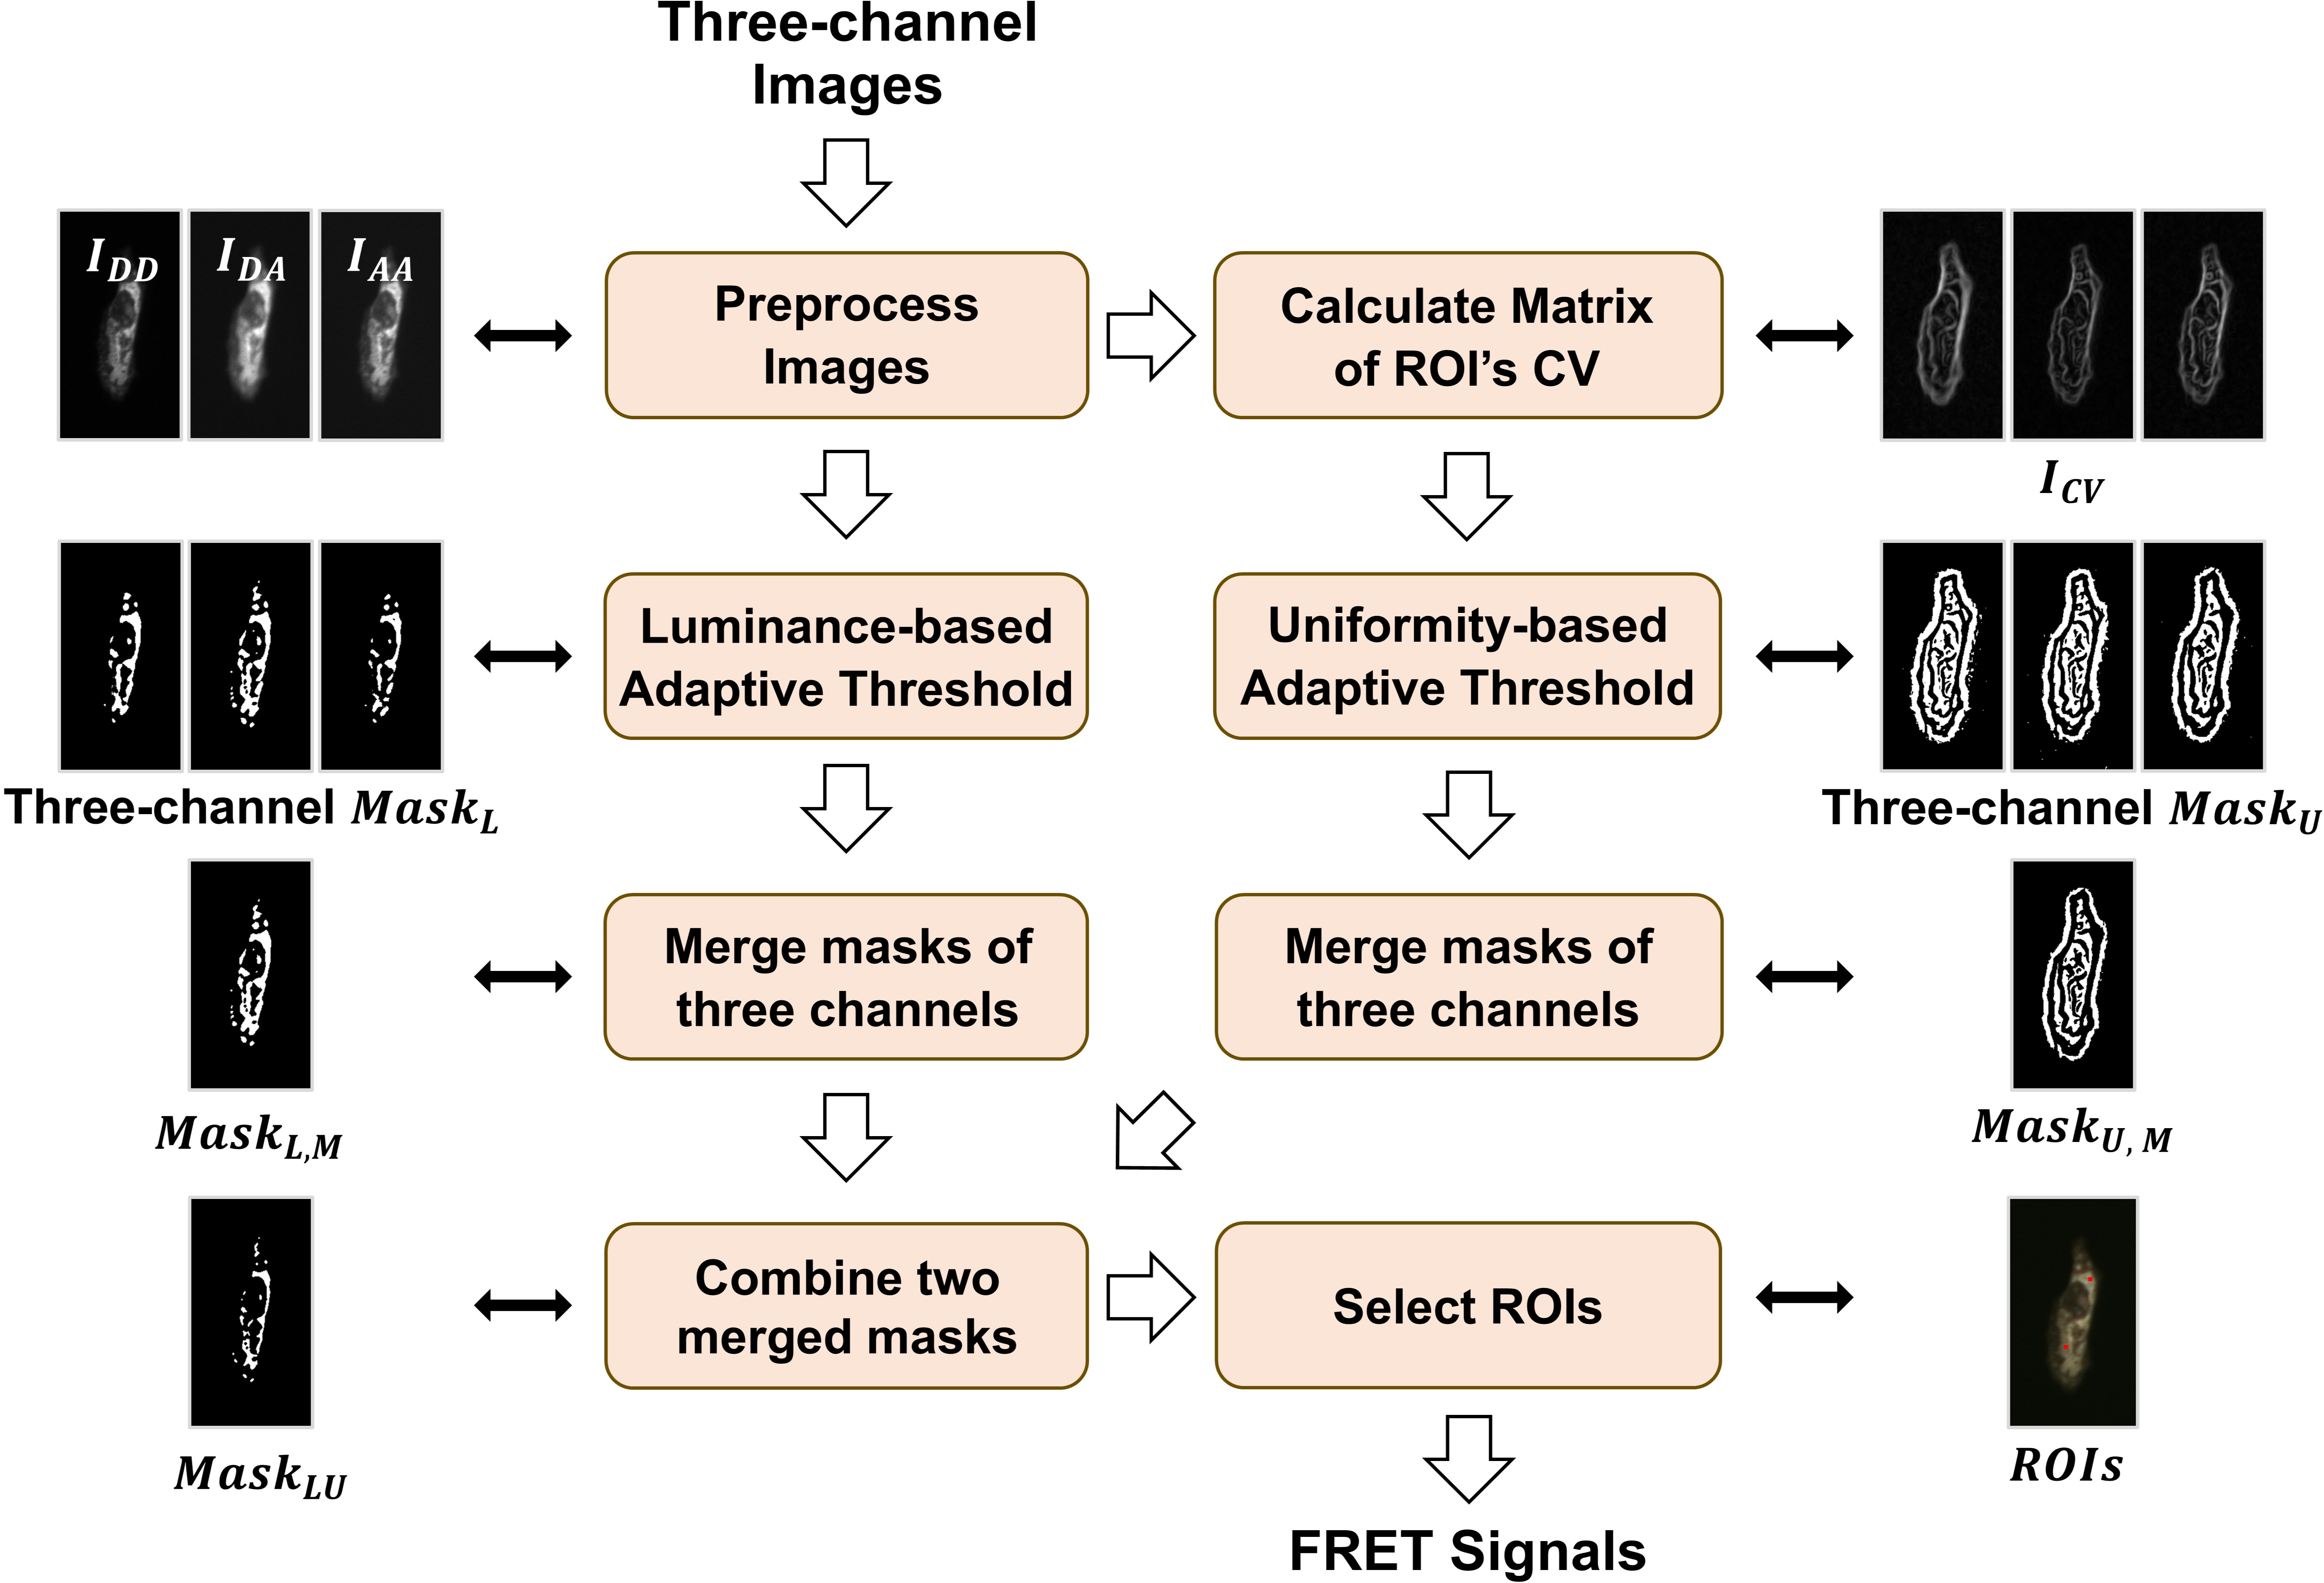
\includegraphics[width=1\linewidth]{../figures/3/3_LURS流程图.png}
\caption{LURS算法流程图}\label{fig1}
\end{figure*}

\subsection{DC-FRET方法的数据范围选取}
\ifshowtext
在应用LURS方法处理FRET双杂交分析数据时,本文更倾向于使用DC-FRET方法而L-FRET方法,因为DC-FRET方法具有以下优势:
\begin{enumerate}
    \item 简化实验过程:与L-FRET方法相比,DC-FRET方法无需在中间分布状态下准备大量样本。相反,仅需准备相对较大$R_C$值和相对较小$R_C$值的样本,这减少了样本的制备和处理时间。
    \item 得出更稳定可靠的结果:DC-FRET中用于线性拟合的供体荧光能量转移效率$E_D$和受供体浓度比$R_C$数据是通过E-FRET和$3^3$-FRET方法进行定量测量的,该方法具有较高的准确性和稳定性,能够提供可靠的数据,使得线性拟合的结果更加稳定可靠。
\end{enumerate}

然而,DC-FRET方法在选择$R_C$或$1/R_C$的范围时需要一定经验。
如果所选范围过小,将会导致数据点不足,从而使结果的稳定性变差。
当拟合范围过大时,结果可能会不正确,因为所选数据不满足尽可能选择受体饱和结合或者供体饱和结合情况。
为了避免使用数据中的不稳定部分,本文中所有自动算法中进行的DC-FRET分析均遵循如下原则:
\begin{enumerate}
    \item 如果样本仅包含供体饱和的情况或仅包含受体饱和的情况,应选择$R_C$($1/R_C$)值相对较小的50\%的数据。
    \item 当受体饱和和供体饱和同时存在时,则应选择$R_C$($1/R_C$)值较小的25\%的数据。
\end{enumerate}

\fi

\section{实验结果}
\subsection{标准质粒验证实验}
准确获取可靠的$3^3$-FRET和 E-FRET的测量结果如供受体视角的FRET效率$E_A$和$E_D$,是成功进行FRET双杂交分析的必要前提。
因此,本文运用LURS方法自动选取ROI,对青色荧光蛋白(CFP)和黄色荧光蛋白(YFP)构建体的单质粒进行了$3^3$-FRET和 E-FRET测量,具体包括 C4Y、C10Y、C40Y 和 C80Y。
这些质粒中的受体和供体的比例均为1:1,但是拥有不同的$E_D$值。
测量的结果列于表\ref{tab:results_standard_plasmids}中。
\begin{table*}[hbtp]
    \centering
    \caption{ 对标准质粒进行$3^3$-FRET和E-FRET测量的结果}
    \begin{tabularx}{\linewidth}{
    >{\centering\arraybackslash}X
    >{\centering\arraybackslash}X
    >{\centering\arraybackslash}X
    >{\centering\arraybackslash}X
    >{\centering\arraybackslash}X
    >{\centering\arraybackslash}X
    >{\centering\arraybackslash}X}
    \toprule
    \multirow{2}{*}{样本} & \multicolumn{3}{c}{测量结果} & \multicolumn{3}{c}{文献结果} \\
     & $E_{A}$ & $E_{D}$ & ${R_C}$ & $E_A$ & $E_{D}$ & $R_C$ \\
    \midrule
    C4Y  & $0.31\pm0.04$ & $0.29\pm0.02$ & $0.98\pm0.11$ & $0.30$ & $0.30$ & $1$ \\
    C10Y & $0.24\pm0.02$ & $0.21\pm0.02$ & $0.94\pm0.10$ & $0.22$ & $0.23$ & $1$ \\
    C40Y & $0.17\pm0.03$ & $0.15\pm0.01$ & $0.98\pm0.17$ & $0.16$ & $0.16$ & $1$ \\
    C80Y & $0.11\pm0.03$ & $0.11\pm0.02$ & $1.03\pm0.20$ & $0.12$ & $0.12$ & $1$ \\
    \bottomrule
    \end{tabularx}
    \label{tab:results_standard_plasmids}
\end{table*}
通过对LURS 提取的ROI的FRET信号进行计算和统计分析,结果表明:C4Y 的$E_D$值为 0.31,C10Y 的$E_D$为 0.23,C40Y 的$E_D$为 0.2,C80Y 的$E_D$为 0.11。
与此同时,C4Y、C10Y、C40Y 和 C80Y 的$R_C$值分别为 0.98、0.94、0.98 和 1.03,与标准值1接近。
所有质粒的$E_D$和$R_C$值都与已报道的值接近,这表明 LURS 算法能够成功提取出正确且有效的ROI,为FRET双杂交分析提供了从供体和受体角度的准确FRET效率数据。

\subsection{模型质粒验证实验}

本文使用LURS结合DC-FRET和L-FRET方法来自动测量各种Cerulean(C,CFP的突变体)和Venus(V,YFP的突变体)构建体的化学计量比,其中包括 C32V 和 CVC。图\ref{fig:results_model_plasmids}展示了共表达 C32V / CVC 且含有游离的 C(C32V + C,CVC + C)(上半部分)或游离的 V(C32V + V,CVC + V)(下半部分)的活 MCF7 细胞的三张荧光图像(DD、AA 和 DA)(左侧),以及由 LURS 生成的ROI(中间),还有DC-FRET和L-FRET的结果图(右侧)。
\begin{figure}[htbp]
    \centering
    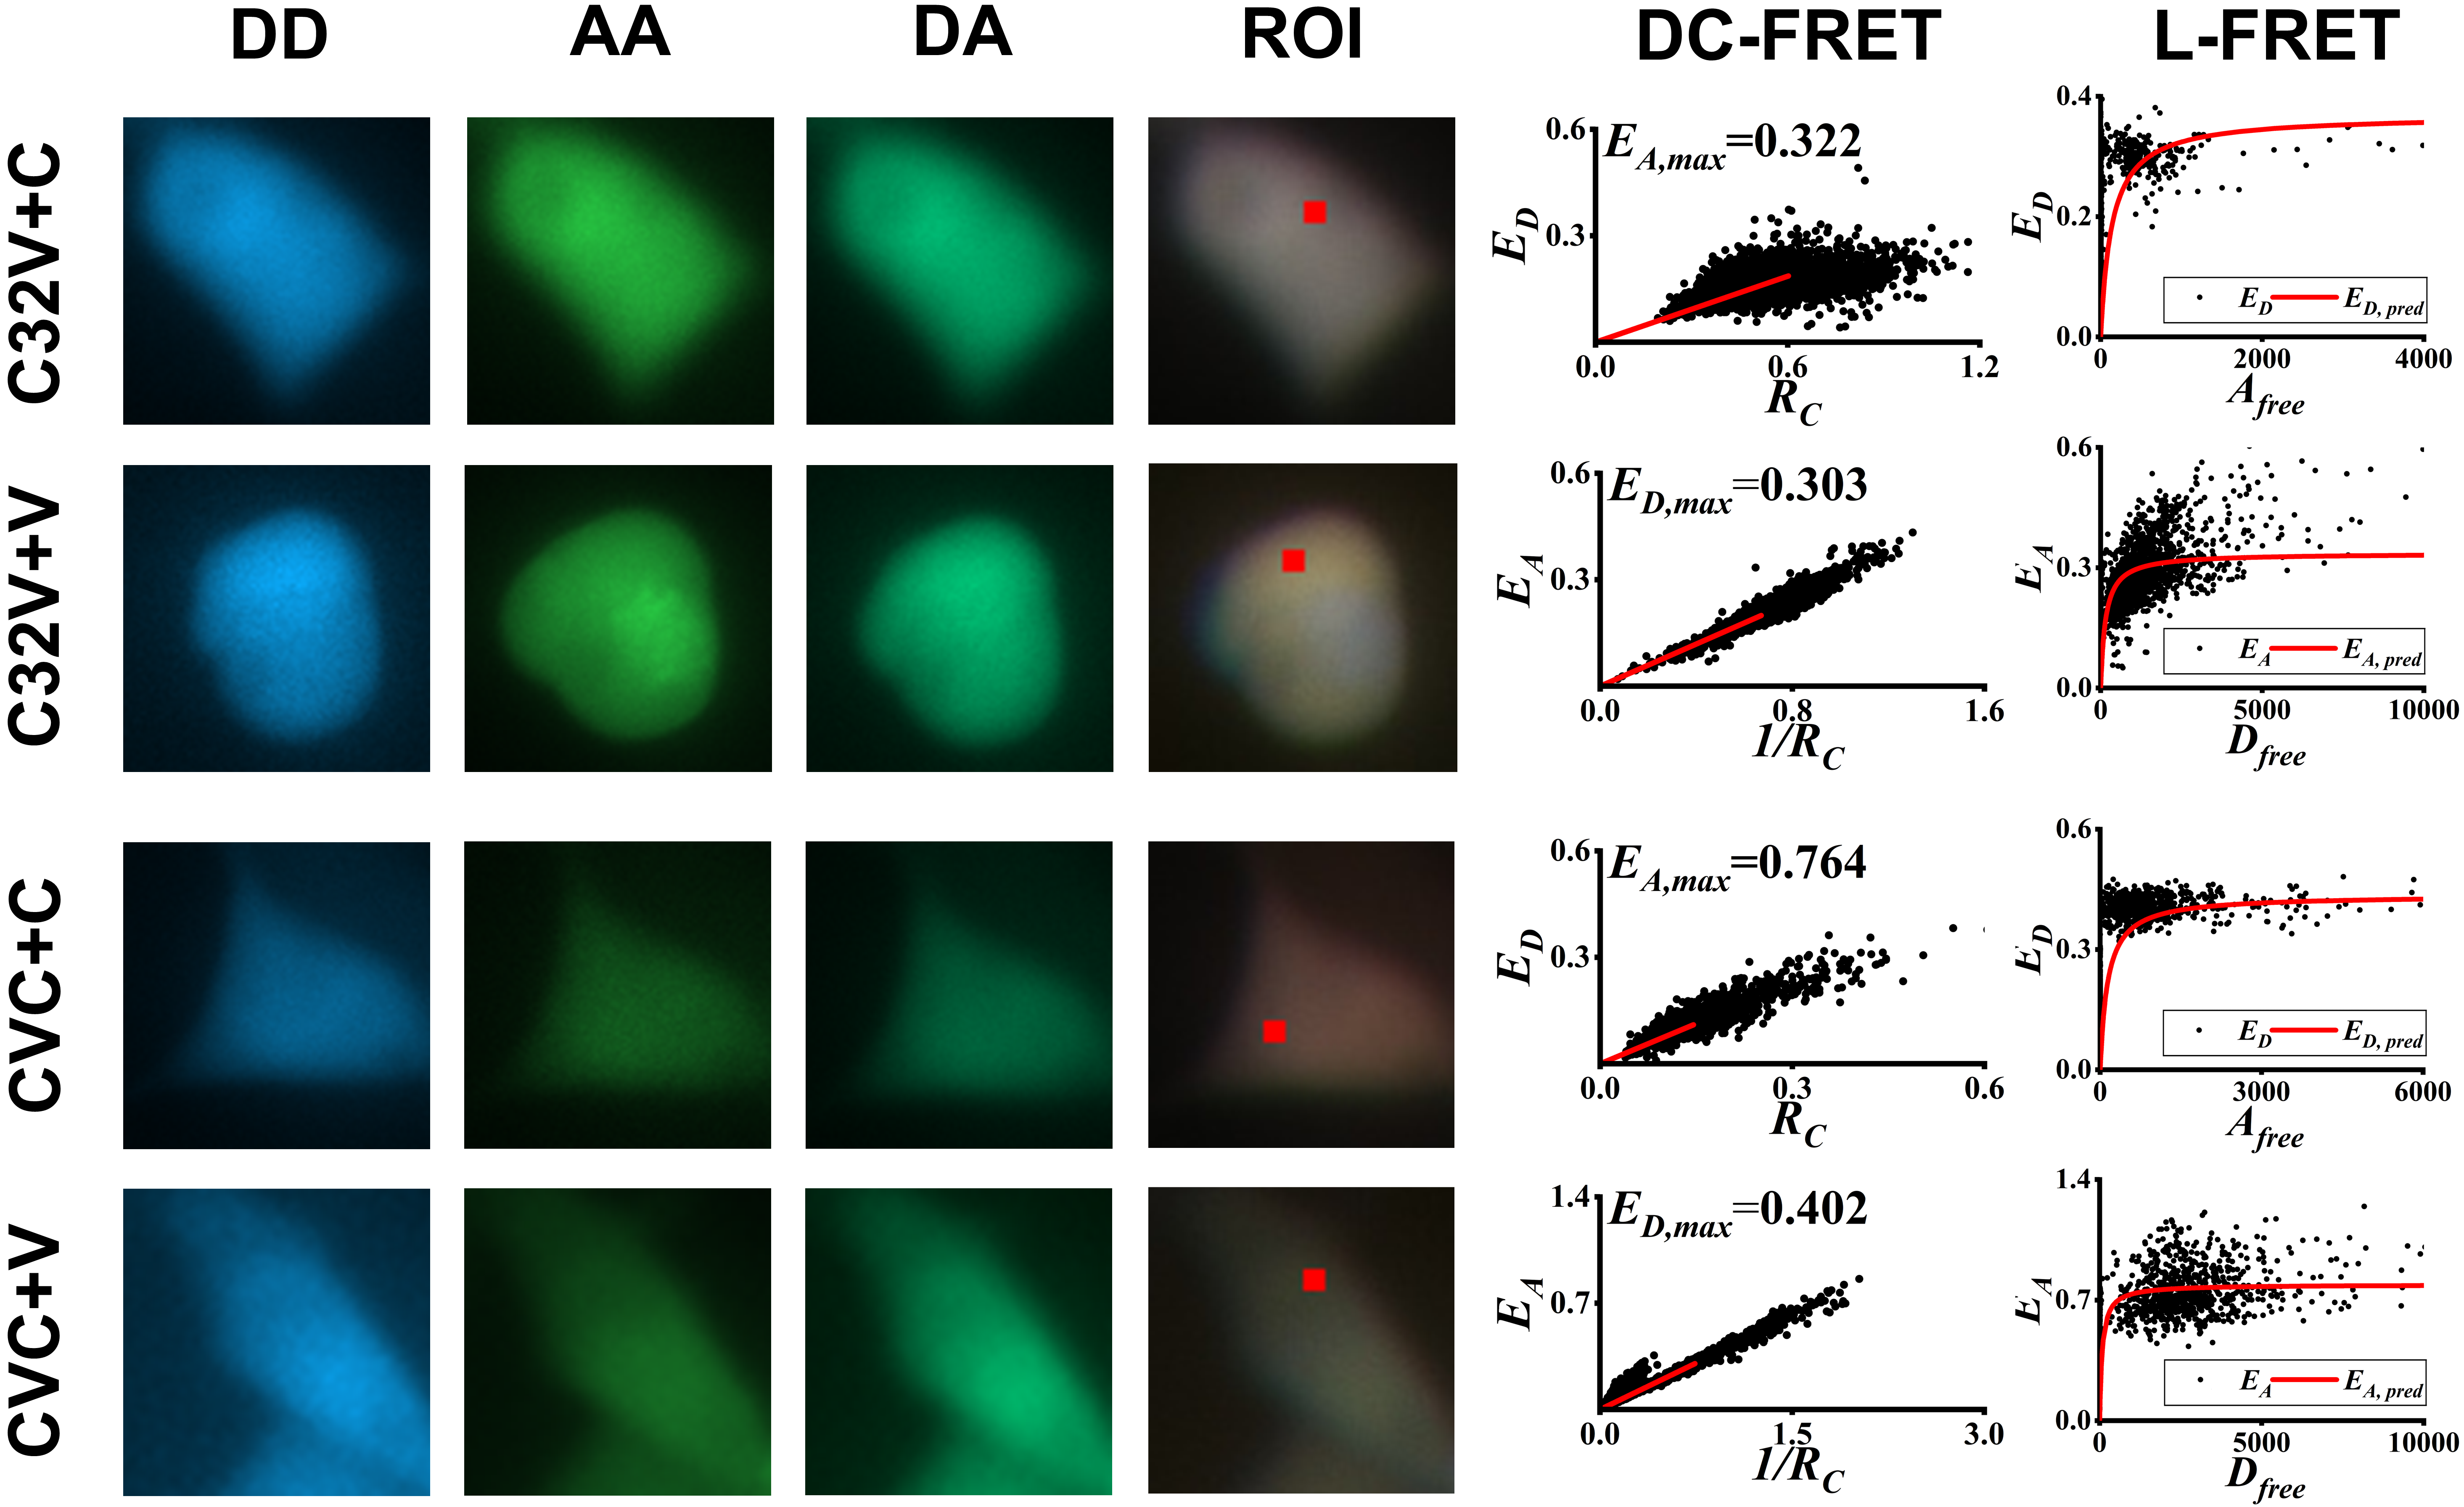
\includegraphics[width=1\linewidth]{../figures/3/LURS模型质粒双杂交.png}
    \caption[模型质粒验证实验结果]{在存在游离供体或受体的情况下,分别通过DC-FRET和L-FRET方法对MCF7活细胞中标准质粒(C32V和CVC)的$E_{A, max}$、$E_{D, max}$和$n_D/n_A$进行自动FRET双杂交分析测量结果。}
    \label{fig:results_model_plasmids}
\end{figure}

C32V 和 CVC 质粒中Cerulean与Venus之间的结合化学计量比的实验测量结果见表\ref{tab:results_model_plasmids}。
LURS结合DC-FRET,测量得到 C32V 质粒中的$E_{A,max}$为 0.322,$E_{D,max}$为 0.303,化学计量比($n_D/n_A$)为 1.063。
这个数值与 C32V 预期的供受体比例1:1非常接近。
对于 CVC 质粒,$E_{A,max}$、$E_{D,max}$和$n_D/n_A$的值分别为 0.764、0.402 和 1.900,所获得的结果与先前文献中报道的结果一致 \upcite{koushik2006cerulean}。
结合L-FRET,LURS自动处理计算得到的 C32V 质粒中的$E_{D,max}$为 0.342,$E_{D,max}$为 0.372,化学计量比($n_D/n_A$)为 0.919。
对于 CVC 质粒,$E_{D,max}$、$E_{D,max}$和$n_D/n_A$的值分别为 0.791、0.442 和 1.790,与文献报道的结果一致 \upcite{thaler2005quantitative}。
这些结果表明,LURS结合DC-FRET和L-FRET方法成功识别到了它们的化学计量比的差别,且计算出的化学计量比和文献结果的相对误差不超过 6\%,进一步证明了LURS算法提取高质量ROI的准确性。

\begin{table*}[htbp]
    \centering
    \caption{模型质粒的FRET双杂交分析结果}
    \begin{tabularx}{\linewidth}{
      >{\centering\arraybackslash}X
      >{\centering\arraybackslash}p{1.8cm}
      >{\centering\arraybackslash}p{1.8cm}
      >{\centering\arraybackslash}p{1.8cm}
      >{\centering\arraybackslash}X
      >{\centering\arraybackslash}X
      >{\centering\arraybackslash}X
      >{\centering\arraybackslash}X
      >{\centering\arraybackslash}X}
      \toprule
      \multirow{2}{*}{样本} & \multicolumn{3}{c}{DC-FRET结果} & \multicolumn{3}{c}{L-FRET 结果} & \multicolumn{2}{c}{文献结果} \\
       & $E_{A,max}$ & $E_{D,max}$ & ${n_D/n_A}$ & $E_{D,max}$ & $E_{D,max}$ & ${n_D/n_A}$ & $E_{D,max}$ & $n_D/n_A$\\
      \midrule
      C32V & $0.322\pm0.041$ & $0.303\pm0.012$ & $1.063\pm0.143$ & $0.342$ & $0.372$ & $0.919$ & 0.311 & 1\\
      CVC  & $0.764\pm0.018$ & $0.402\pm0.024$ & $1.900\pm0.113$ & $0.791$ & $0.442$ & $1.790$ & 0.414 & 2\\
      \bottomrule
      \hline %
      \end{tabularx}
    \label{tab:results_model_plasmids}
\end{table*}

\subsection{活细胞中 Bcl-xL-Bak 化学计量比的自动分析}

接下来,为了研究选择性 Bcl-xL 抑制剂 A1331852 存在下的 Bcl-xL-Bak 相互作用,本文将LURS算法应用于测量两者化学计量比变化的活细胞实验 \upcite{wang2020discovery}。

为了对比LURS自动ROI提取算法和深度学习方法的效果,本文分别测试了应用ilastik的方法、应用SAM-Med2D的方法进行了自动数据处理,然后对比了不同方法的精确度和对药物敏感度的测试。
在图像处理和ROI上,基于ilastik的方法通过手动对图像进行交互式标注,对输入的10个视野30张荧光细胞图像进行标注,将图像的像素分类为好细胞、坏细胞和背景区域,然后应用训练后的ilastik的模型进行自动分割,完成了对ROI的选取。
基于SAM-Med2D的方法通过手动对图像进行标注,标注了好细胞和背景区域,然后分别作为大模型输入的提示词(prompt)进行提示,然后输入实验数据完成自动分割。
在FRET双杂交分析方法上,由于DC-FRET的稳定性,本文选取DC-FRET作为分析模型和方法。

首先,如图 \ref {fig3} 所示,所有方法均能高精度测量 FRET 效率及化学计量比,并有效检测药物处理前后的参数显著变化。
这些结果表明,A1331852可破坏 Bcl-xL/Bak 相互作用,导致 受体中心的FRET 效率、供体中心的FRET效率和化学计量比均显著降低,且与手动分析结果趋势一致,验证了不同方法的测量一致性。

\begin{figure*}[!htb]
  \centering
  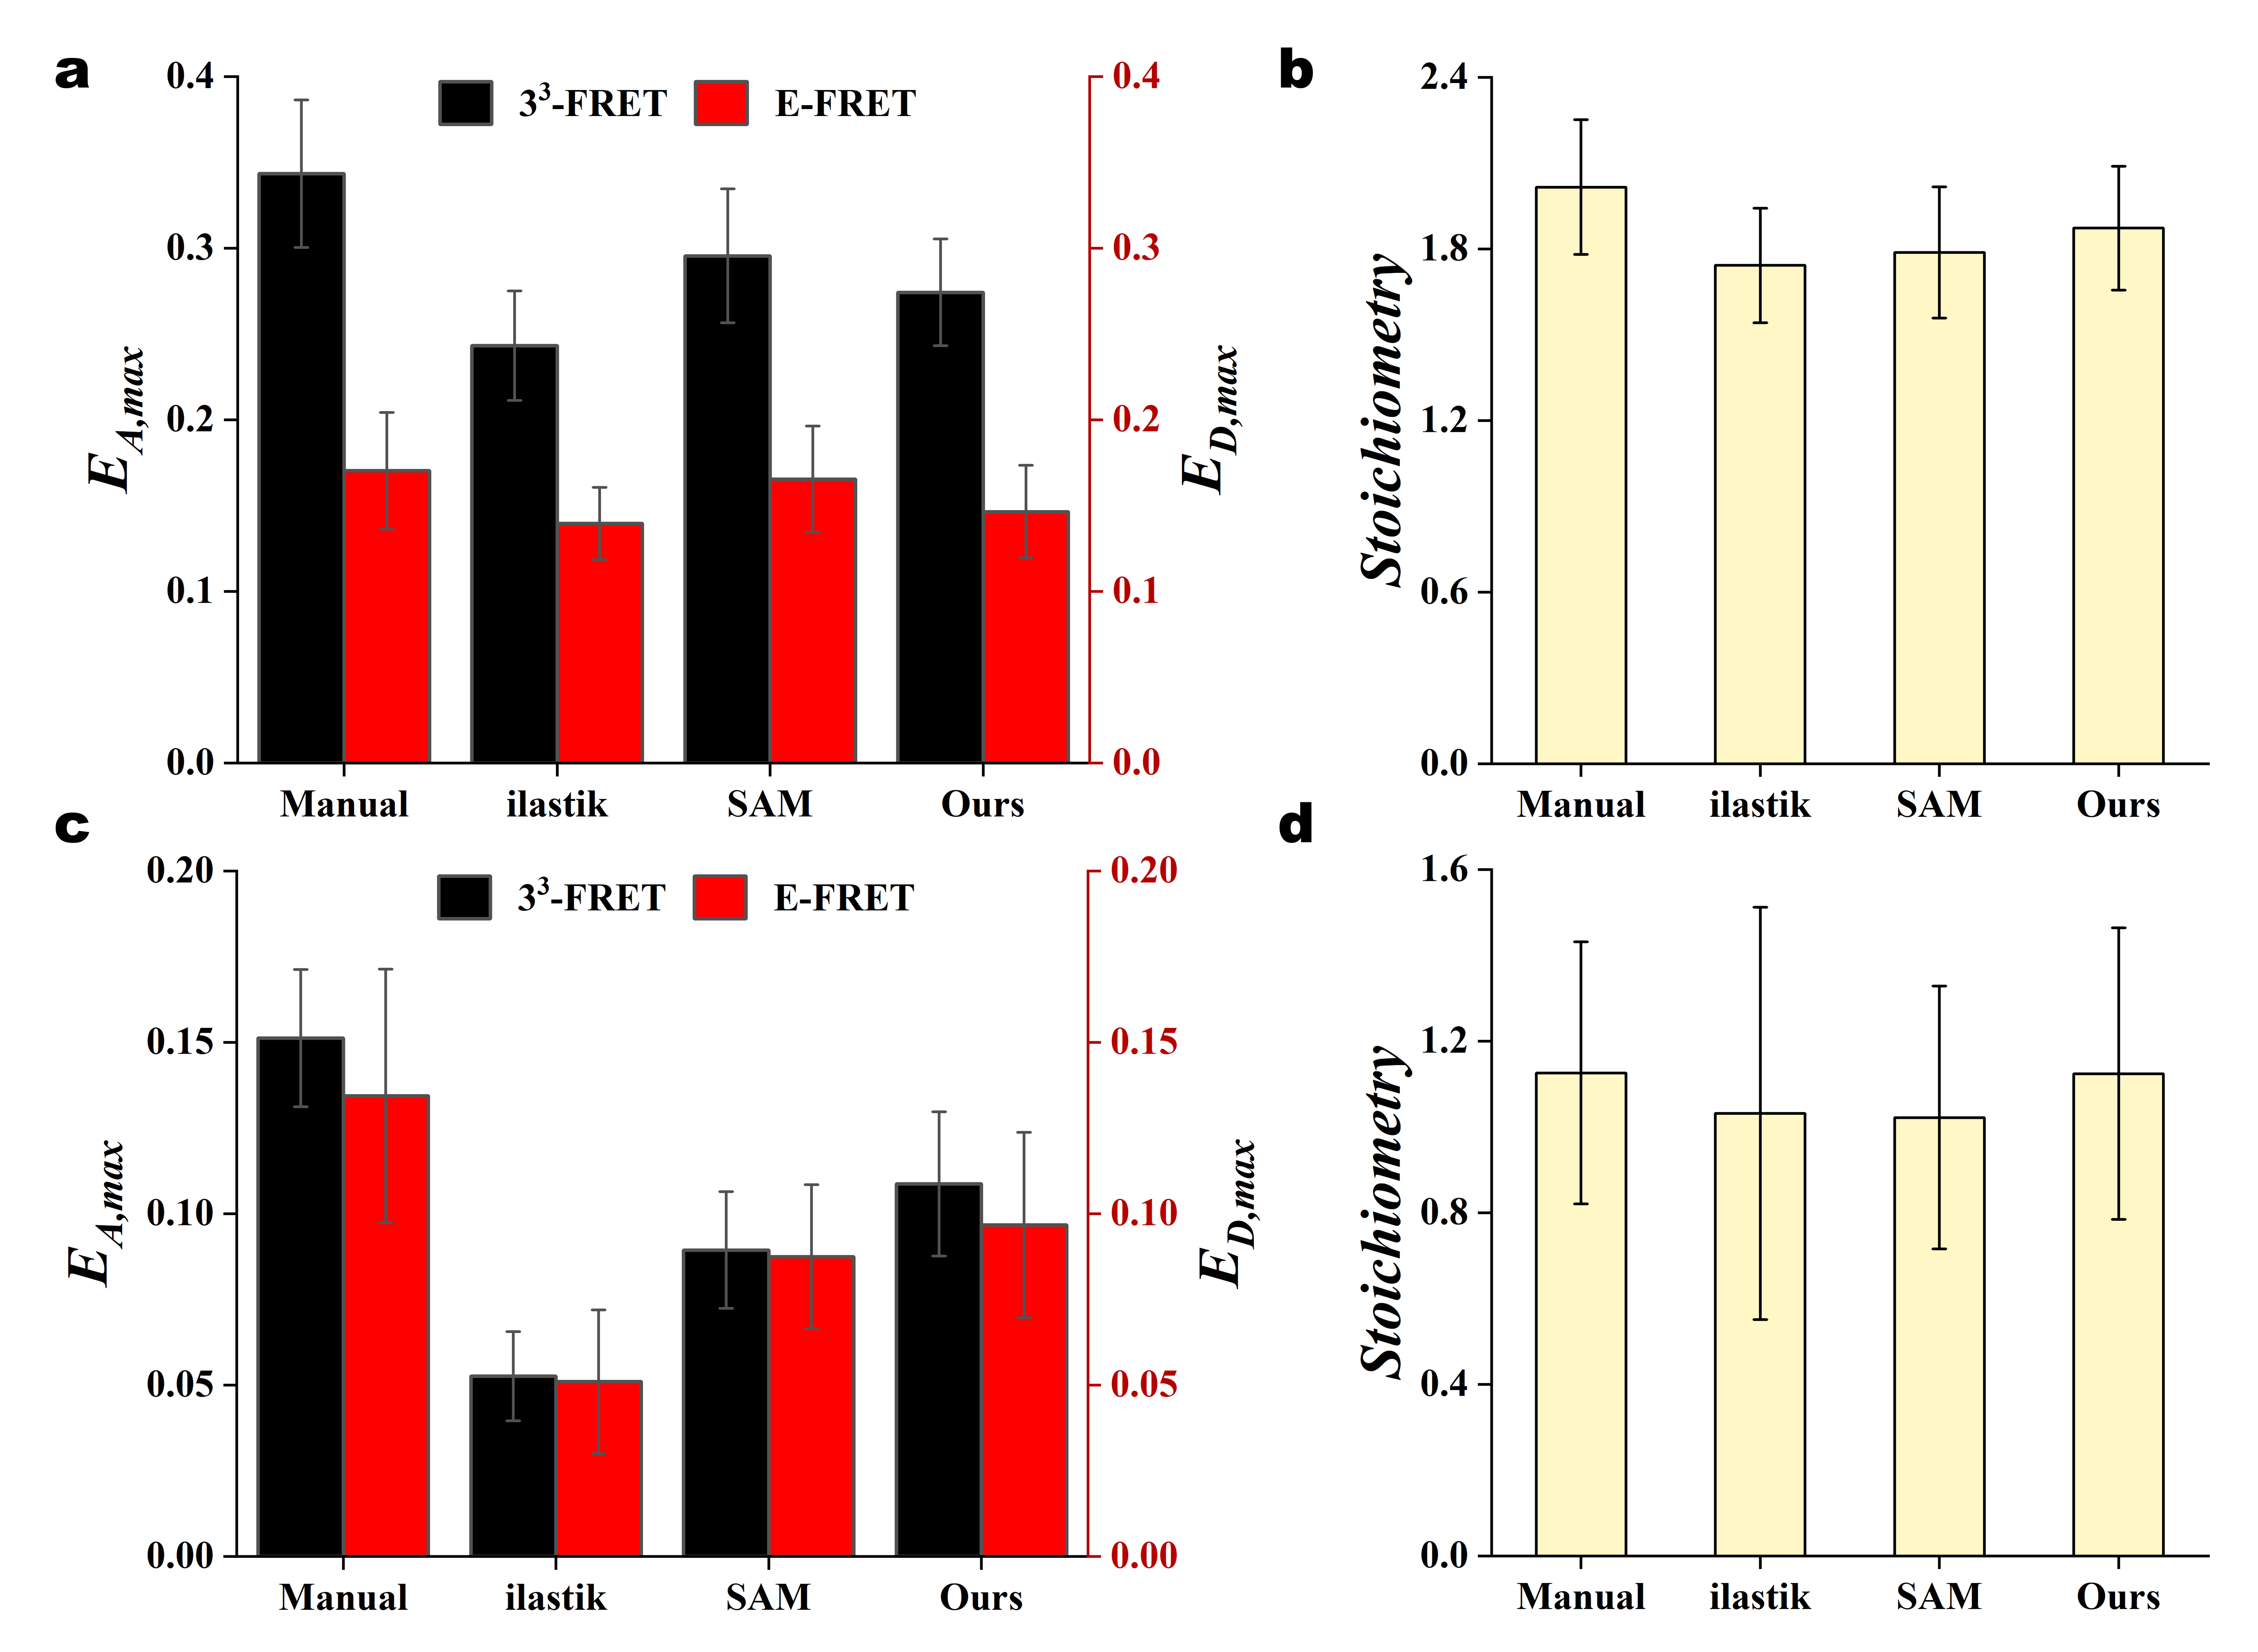
\includegraphics[width=1\linewidth]{../figures/4/4_方法对比.png}
  \caption[活细胞中 Bcl-xL-Bak 化学计量比的自动分析方法对比]{活细胞中 Bcl-xL-Bak 化学计量比的自动分析方法对比。手动、ilastik、SAM-Med2D及本方法计算的,A1331852处理前(a,b)和处理后(c,d)Bcl-xL-CFP与Bak-YFP结合的最大$3^3$-FRET(黑色)和E - FRET(红色)效率以及化学计量比(黄色)。}\label{fig3}
\end{figure*}

其次,本方法在FRET参数测量中表现出优于SAM-Med2D和ilastik的整体准确性(表 \ref{tab:comparison})。
对照组中,本方法测得$E_{A,{max}}=0.27\pm0.03$、$E_{D,{max}}=0.15\pm0.03$。尽管SAM-Med2D的$E_{A,{max}}$($0.29\pm0.04$)更接近手动值($0.34\pm0.04$),但本方法在$E_{D,{max}}$($0.15\pm0.03$ vs 手动$0.17\pm0.03$)和化学计量比($n_D/n_A=1.87\pm0.22$)上偏差最小(手动$2.01\pm0.14$),而SAM-Med2D($1.79\pm0.33$)和ilastik($1.74\pm0.19$)的化学计量比偏离更显著。
在A1331852处理组中,本方法的所有参数均最贴近手动结果:$E_{A,{max}}=0.11\pm0.02$、$E_{D,{max}}=0.10\pm0.03$(手动$0.15\pm0.02$、$0.13\pm0.04$),显著优于SAM-Med2D($0.09\pm0.02$)和ilastik($0.05\pm0.01$)。特别值得注意的是,本方法的化学计量比$n_D/n_A=1.12\pm0.33$与手动结果($1.12\pm0.30$)完全一致,而SAM-Med2D($1.02\pm0.30$)和ilastik($1.03\pm0.48$)表现出更大离散性。这些结果突显了本方法在扰动条件下定量FRET效率与化学计量比的稳健性。

\begin{table*}[htbp]
  \centering
  \caption[活细胞中 Bcl-xL-Bak 化学计量比的自动分析方法对比]{手动、基于ilastik、基于SAM-Med2D 及Fretha自动方法测量 A1331852 处理前后 Bcl-xL-CFP 与 Bak-YFP 结合的 DC-FRET 双杂交分析结果。}
  \begin{tabularx}{\linewidth}{
  >{\centering\arraybackslash}p{2.2cm}
  >{\centering\arraybackslash}X
  >{\centering\arraybackslash}X
  >{\centering\arraybackslash}X
  >{\centering\arraybackslash}X
  >{\centering\arraybackslash}X
  >{\centering\arraybackslash}X}
  \toprule
  \multirow{2}{*}{方法} & \multicolumn{3}{c}{对照组} & \multicolumn{3}{c}{加药组}  \\
   & $E_{A,max}$ & $E_{D,max}$ & ${n_D/n_A}$ & $E_{D,max}$ & $E_{D,max}$ & ${n_D/n_A}$ \\
  \midrule
  Manual    & $0.34\pm0.04$ & $0.17\pm0.03$ & $2.01\pm0.14$ & $0.15\pm0.02$ & $0.13\pm0.04$ & $1.12\pm0.30$ \\
  ilastik   & $0.24\pm0.03$ & $0.14\pm0.02$ & $1.74\pm0.19$ & $0.05\pm0.01$ & $0.05\pm0.02$ & $1.03\pm0.48$ \\
  SAM-Med2D & $0.29\pm0.04$ & $0.17\pm0.05$ & $1.79\pm0.33$ & $0.09\pm0.02$ & $0.09\pm0.02$ & $1.02\pm0.30$ \\
  Ours      & $0.27\pm0.03$ & $0.15\pm0.03$ & $1.87\pm0.22$ & $0.11\pm0.02$ & $0.10\pm0.03$ & $1.12\pm0.33$ \\
  \bottomrule
  \hline %
  \end{tabularx}
  \label{tab:comparison}
\end{table*}

\subsection{LURS算法性能分析}
在相同硬件配置(Intel\textsuperscript{\textregistered} Xeon E5-2678 v3 @ 2.50GHz处理器,NVIDIA\textsuperscript{\textregistered} GeForce RTX 3090 GPU)下,我们对LURS算法与两种基于深度学习的自动ROI提取方法(ilastik和SAM-Med2D)进行了系统性性能对比。

如表 \ref{tab:性能对比} 所示,LURS方法在1.4GB数据集(包含30个视野的药物处理组和对照组)中仅需10秒即可提取1515个可用的ROI,单ROI处理时间低至6.6 ms。
相比之下,ilastik和SAM-Med2D的单ROI处理时间分别为35.2 ms和50.7 ms,LURS的速度较ilastik提升5.3倍,较SAM-Med2D提升7.7倍。  

内存利用率方面,LURS仅占用约800 MB内存,分别为ilastik(~1.8 GB)的44\%和SAM-Med2D(~14 GB)的5.7\%。这一优化使得LURS在资源受限的环境中仍能高效运行。
此外,LURS完全依赖CPU资源,无需专用GPU加速,使其能够直接集成到实时显微镜成像系统中,为高通量筛选应用提供了硬件无关性和部署灵活性。  

上述结果表明,LURS在处理速度、内存效率和硬件适应性方面展现出显著优势。LURS算法在保证数据处理精度的同时,通过集成在Fretha软件系统中进行统一数据模型管理,优化计算流程和内存管理,显著提升了处理效率并降低了硬件依赖,为实时、高通量的FRET数据分析提供了更优的解决方案。

\begin{table*}[htbp]
    \centering
    \caption{不同算法的性能对比}
    \begin{tabular}{cccc}
    \toprule[1.5pt]
    方法 & 单ROI处理时间(ms) & 内存占用 & 硬件依赖 \\
    \midrule
    LURS & 6.6 & ~800 MB & CPU \\
    ilastik & 35.2 & ~1.8 GB & GPU/CPU \\
    SAM-Med2D & 50.7 & ~14 GB & GPU \\
    \bottomrule[1.5pt]
    \end{tabular}
    \label{tab:性能对比}
\end{table*}

\section{本章小结}

\ifshowtext
本章针对传统 FRET 双杂交分析中数据处理效率低、质量依赖人工标注等问题,提出基于亮度均匀性的 ROI 选择算法(LURS)。
该算法通过高斯平滑预处理、多通道自适应阈值分割和变异系数均匀性评估,实现了荧光信号的高效提取。
结合 DC-FRET 方法的自动数据范围选取策略,该系统成功实现了 FRET 双杂交分析的全流程自动化,为高通量药物筛选和蛋白质互作研究提供了可靠的技术支撑,丰富了数据处理软件Fretha的功能。
实验结果表明,LURS 算法在标准质粒 C4Y/C10Y/C40Y/C80Y 的 E-FRET 测量中,$E_A$ 与 $E_D$ 值与文献报道误差小于 5\%,RC 值偏差不超过 0.05,验证了算法的准确性。
在模型质粒 C32V 和 CVC 的化学计量比分析中,测量的 $n_D/n_A$ 值分别为 1.06 ± 0.14 和 1.90 ± 0.11,与理论值 1:1 和 2:1 高度吻合,且计算效率较人工处理提升 80\% 以上。
应用自动算法分析活细胞中Bcl-xL-Bak之间的相互作用表明,LURS结合DC-FRET算法敏锐地检测到Bcl-xL和Bak之间的作用计量从1.87下降到1.12,在ilastik、SAM-Med2D等方法中最接近人工手动处理的标准结果。
这些结果表明,LURS算法在FRET双杂交分析数据处理中具有较高的准确性和稳定性,为高通量药物筛选和蛋白质互作研究提供了可靠的技术支撑。
\fi